\subsection{Angle Bisectors}
\renewcommand{\theequation}{\theenumi}
\begin{enumerate}[label=\arabic*.,ref=\thesubsection.\theenumi]
\numberwithin{equation}{enumi}
\item
	In Fig. \ref{ch3_angle_bisector}, $OB$ divides the  $\angle B$ into half, i.e.\begin{equation}
	\angle OBC = \angle OBA
	\end{equation}
	$OB$ is known as an angle bisector.


\begin{figure}[!ht]
	\begin{center}
		
		%
\includegraphics[width=\columnwidth]{./figs/ch3_angle_bisector}
		%\vspace*{-10cm}
%		\resizebox{\columnwidth}{!}{\begin{tikzpicture}
[scale=2,>=stealth,point/.style={draw,circle,fill = black,inner sep=0.5pt},]

\node (D) at (0, 0)[point,label=below :$D$] {};
\node (A) at (0, 3)[point,label=above :$A$]{};
\node (B) at (-3, 0)[point,label=below left:$B$]{};
\node (C) at (3, 0)[point,label=below right:$C$]{};
\node (O) at (0, 1.3)[point,label=below right:$O$]{};
\node (F) at (-1.1, 1.9)[point,label=above left:$F$]{};
\node (E) at (1.1, 1.9)[point,label=above right:$E$]{};

\draw (D)--(B);
\draw (B)--(A);
\draw (A)--(C);
\draw (C)--(D);
\draw [thick,dashed] (A) -- (D);
\draw [thick,dashed] (O) -- (E);
\draw [thick,dashed] (O) -- (F);
\draw (B)--(O);
\draw (C)--(O);

\tkzMarkRightAngle[size=.2](A,D,C)
\tkzMarkRightAngle[size=.15](B,F,O);
\tkzMarkRightAngle[size=.15](C,E,O);
\tkzMarkAngle[size=.4](D,B,O);
\tkzMarkAngle[size=.35](O,B,F);
\tkzMarkAngle[size=.54](E,C,O);
\tkzMarkAngle[size=.5](E,C,O);
\tkzMarkAngle[size=.6](O,C,D);
\tkzMarkAngle[size=.65](O,C,D);

\end{tikzpicture}}
%		\resizebox{\columnwidth}{!}{\begin{tikzpicture}
[
 scale=2,
  >=stealth,
  point/.style = {draw, circle, fill = black, inner sep = 1pt},
]

\node (B) at (-2,-2)[point,label = below left:${B}$] {};
\node (A) at (1,3)[point,label = above left:${A}$] {};
\node (C) at (4,-1)[point,label = below right:${C}$] {};
\draw (A) -- (B) -- (C) -- (A);

\node (D) at (2.4682957,1.0422724)[point,label = above right:$D$] {};
\draw (B) -- (D);


\node (E) at (1.23016035,-1.46163994)[point,label = below:$E$] {};
%\draw (A) -- (E);
\draw[thick, dashed] (A) -- (E);


\node (F) at (-0.35345316,  0.74424473)[point,label = left:$F$] {};
\draw (C) -- (F);

\node (O) at (1.14738665, 0.14292163) [point,label = right:$O$] {};

\tkzMarkAngle[fill=blue!60,size=.3](O,B,F)
\tkzMarkAngle[fill=blue!40,size=.3](E,B,O)


\tkzMarkAngle[fill=red!60,size=.3](F,A,O)
\tkzMarkAngle[fill=red!40,size=.3](O,A,D)


\tkzMarkAngle[fill=orange!60,size=.3](D,C,O)
\tkzMarkAngle[fill=orange!40,size=.3](O,C,E)


\end{tikzpicture}}
		\resizebox{\columnwidth}{!}{\begin{tikzpicture}
[
 scale=2,
  >=stealth,
  point/.style = {draw, circle, fill = black, inner sep = 1pt},
]

\node (B) at (-2,-2)[point,label = below left:${B}$] {};
\node (A) at (1,3)[point,label = above left:${A}$] {};
\node (C) at (4,-1)[point,label = below right:${C}$] {};
\draw (A) -- (B) -- (C) -- (A);
\node (O) at (1.14738665, 0.14292163) [point,label = right:$O$] {};

\node (D) at (1.40982295, -1.43169617)[point,label = below right:$D$] {};
\draw (O) -- (D);

\node (E) at (2.42445681, 1.10072425)[point,label = below:$E$] {};
\draw (O) -- (E);
%\draw[thick, dashed] (A) -- (E);


\node (F) at (-0.22146164,  0.9642306)[point,label = left:$F$] {};
\draw (O) -- (F);
\draw (O) -- (C);
\draw (O) -- (B);
\draw[thick, dashed] (A) -- (O);
%\draw (O) -- (A);


\tkzMarkAngle[fill=blue!60,size=.3](O,B,F)
\tkzMarkAngle[fill=blue!40,size=.3](D,B,O)


\tkzMarkAngle[fill=red!60,size=.3](F,A,O)
\tkzMarkAngle[fill=red!40,size=.3](O,A,E)


\tkzMarkAngle[fill=orange!60,size=.3](E,C,O)
\tkzMarkAngle[fill=orange!40,size=.3](O,C,D)

\tkzMarkRightAngle[fill=blue!20,size=.3](A,E,O)
\tkzMarkRightAngle[fill=blue!20,size=.3](A,F,O)
\tkzMarkRightAngle[fill=blue!20,size=.3](O,D,C)

%\def\rad{1.596337700952456}
%%\coordinate [point, label={above : $O$ }] (O) at (0, 0);
%\draw (O) circle (\rad);

\end{tikzpicture}
}
	\end{center}
	\caption{Angle bisectors meet at a point}
	\label{ch3_angle_bisector}	
\end{figure}

	$OB$ and $OC$ are angle bisectors of angles $B$ and $C$. $OA$ is joined and $OD, OF$ and $OE$ are perpendiculars to sides $a,b$ and $c$.
\item
  Show that $OD = OE = OF$.
\solution In $\triangle$s $ODC$ and $OEC$,
\begin{align}
OD &= OC \sin \frac{C}{2}
\\
OE &= OC \sin \frac{C}{2} 
\\
\Rightarrow OD &=OE.
\end{align}
Similarly,
\begin{equation}
OD = OF.
\end{equation}
%
\item
	Show that OA is the angle bisector of $\angle A$
\\
\solution In $\triangle$s $OFA$ and $OEA$,
\begin{align}
OF &= OE
\\
\Rightarrow OA \sin OAF &= OA \sin OAE \\
\Rightarrow \sin OAF &=  \sin OAE \\
\Rightarrow \angle OAF &= \angle OAE
\end{align}
which proves that $OA$ bisects $\angle A$.
\\
{\em Conclusion:} The angle bisectors of a triangle meet at a point.
\item If $OD=OE=OF=r$, find $r$ in terms of $a,b,c$.
\end{enumerate}
\subsection{Congruent Triangles}
%
\renewcommand{\theequation}{\theenumi}
\begin{enumerate}[label=\arabic*.,ref=\thesubsection.\theenumi]
\numberwithin{equation}{enumi}

\item
	Show that in $\triangle$s $ODC$ and $OEC$, corresponding sides and angles are equal.  Such triangles are known as {\em congruent} triangles and denoted by $\triangle ODC \cong \triangle OEC$.

\item
To show that two triangles are congruent, it is sufficient to show that some angles and sides are equal.  

\item
SSS:	Show that if the corresponding sides of three triangles are equal, the triangles are congruent.

\item
ASA:	Show that if two angles and any one side  are equal in corresponding triangles, the triangles are congruent.

\item
SAS:	Show that if two sides and the angle between them are equal in corresponding triangles, the triangles are congruent.

\item
RHS:	For two right angled triangles, if the hypotenuse and one of the sides are equal, show that the triangles are congruent.
\end{enumerate}

	%
%%
\subsection{Perpendicular Bisectors}
\renewcommand{\theequation}{\theenumi}
\begin{enumerate}[label=\arabic*.,ref=\thesubsection.\theenumi]
\numberwithin{equation}{enumi}

\item
	In Fig. \ref{ch3_perp_bisector}, $OE \perp AC, OF \perp AB, AE=EC, AF=FB$.  $OE$ and $OF$ are known as the {\em perpendicular bisectors} of $AC$ and $AB$ respectively.  Show that $OA=OB=OC$.
%
\\
\solution Using SAS, $\triangle OEA \cong \triangle OEC$.  Thus, $OA = OC$.  Similarly,   $\triangle OFA \cong \triangle OFB \implies OA = OB$.

\item
	In Fig. \ref{ch3_perp_bisector}, show that if $OD \perp BC$, $BD=DC$, i.e., $OD$ is the perpendicular bisector of $BC$.
.
\\
\solution $\because OB = OC$, using RHS congruence, $\triangle ODC \cong \triangle ODB$.  Hence $BD = DC$.\item
	In Fig. \ref{ch3_perp_bisector}, show that if $BD=DC$, $OD \perp BC$.
.
\\
\solution Use SSS.
%%
%%
\begin{figure}[!ht]
	\begin{center}
		
%		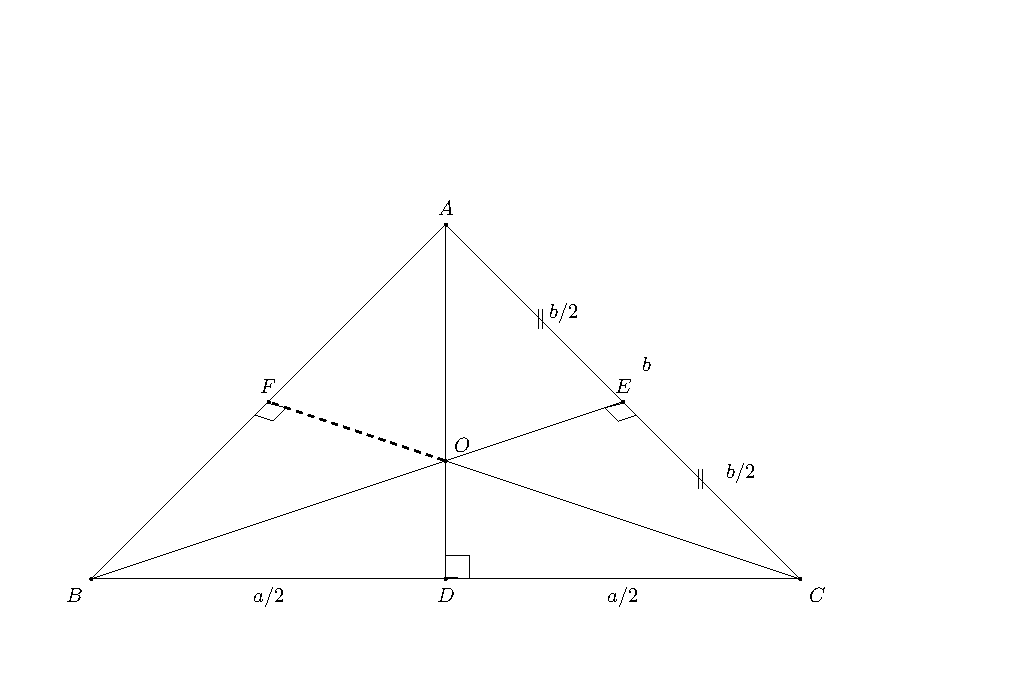
\includegraphics[width=\columnwidth]{./figs/fig_3.8.eps}
		\resizebox{\columnwidth}{!}{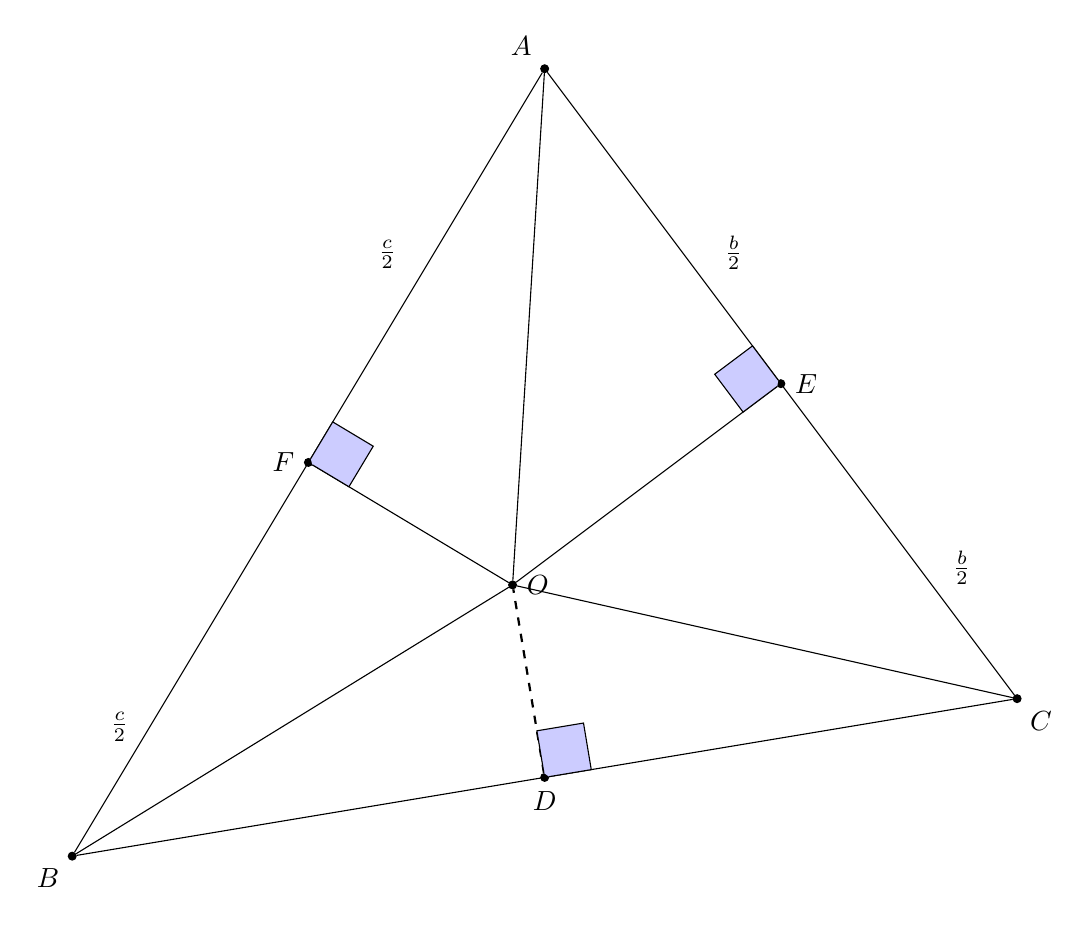
\begin{tikzpicture}
[
 scale=2,
  >=stealth,
  point/.style = {draw, circle, fill = black, inner sep = 1pt},
]
\node (B) at (-2,-2)[point,label = below left:${B}$] {};
\node (A) at (1,3)[point,label = above left:${A}$] {};
\node (C) at (4,-1)[point,label = below right:${C}$] {};
\draw (A) -- (B) -- (C) -- (A);

\node (D) at (1,-1.5)[point,label = below:$D$] {};

\node (F) at (-0.5,0.5)[point,label = left:$F$] {};

\node (E) at (2.5,1)[point,label = right:$E$] {};

\node (O) at (0.7962963,-0.27777778) [point,label = right:$O$] {};

\draw[thick, dashed] (D) -- (O);
\draw (F) -- (O);
\draw (E) -- (O);
\draw (A) -- (O);
\draw (B) -- (O);
\draw (C) -- (O);

\tkzMarkRightAngle[fill=blue!20,size=.3](A,E,O)
\tkzMarkRightAngle[fill=blue!20,size=.3](A,F,O)
\tkzMarkRightAngle[fill=blue!20,size=.3](O,D,C)


\node [below] at (3.65,0) {\strut $\frac{b}{2}$};
\node [below] at (2.2,2) {\strut  $\frac{b}{2}$};


%\node [below] at (2.5,-1.2) {\strut a/2};    
%\node [below] at (0,-1.65) {\strut a/2};  
      
\node [below] at (-1.7,-1) {\strut  $\frac{c}{2}$}; 
\node [below] at (0,2) {\strut  $\frac{c}{2}$};   


\end{tikzpicture}
}
%		\includegraphics[width=\columnwidth]{./figs/fig26_def}
		%\vspace*{-10cm}
%		\resizebox{\columnwidth}{!}{\documentclass{standalone}
\usepackage{tikz}
\usepackage{tkz-euclide}
\usetkzobj{all}
%\usepackage{amsmath}
\providecommand{\brak}[1]{\ensuremath{\left(#1\right)}}

\begin{document}
\begin{tikzpicture}
[scale=2,>=stealth,point/.style={draw,circle,fill = black,inner sep=0.5pt},]

\node (E) at (1.5, 1.5)[point,label=above :$E$] {};
\node (F) at (-1.5, 1.5)[point,label=above :$F$] {};
\node (A) at (0, 3)[point,label=above :$A$]{};
\node (B) at (-3, 0)[point,label=below left:$B$]{};
\node (C) at (3, 0)[point,label=below right:$C$]{};
\node (D) at (0,0)[point,label=below :$D$] {};
\node (O) at (0,1)[point,label=above right :$O$] {};


\draw (B)--(A);
\draw (A)--(C);
\draw (B)--(C);
\draw (B)--(E);
\draw (C)--(O);
\draw (A)--(D);
\draw [thick,dashed] (O) -- (F);

\node [above] at (1.7,1.7) {$b$};
\node [above] at (2.5,.75) {$b/2$};
\node [above] at (1,2.1) {$b/2$};
\node [above] at (-1.5,-0.3){$a/2$};
\node [above] at (1.5,-0.3){$a/2$};
\tkzMarkRightAngle[size=.16](B,F,O)
\tkzMarkRightAngle[size=.16](C,E,O)
\tkzMarkRightAngle[size=.2](A,D,C)
\draw   -- (4.3,1.7) node[midway] {$\parallel$};
\draw   -- (1.6,4.4) node[midway] {$\parallel$};

\end{tikzpicture}
\end{document}}
	\end{center}
	\caption{Perpendicular bisectors meet at a point}
	\label{ch3_perp_bisector}	
\end{figure}
%
%\solution In $\triangle$s $ODB$ and $ODC$, using Budhayana's theorem,
%%
%\begin{equation}
%\begin{split}
%OB^2 &= OD^2 + BD^2 \\
%OC^2 &= OD^2 + DC^2 
%\end{split}
%\end{equation}
%
%Since $BD = DC = \frac{a}{2}$, $OB = OC$.  Similarly, it can be shown that $OA = OC$.  Thus, $OA=OB=OC$.
%
\item
	In $\triangle AOB$, $OA = OB$.  Such a triangle is known as an isoceles triangle.
%
%\item
%	Show that $AF = BF$.
%
%\solution Trivial using Budhayana's theorem.  This shows that $OF$ is a perpendicular bisector of $AB$. 
\\
{\em Conclusion:}  The perpendicular bisectors of a triangle meet at a point.
%
\item In Fig. \eqref{ch3_perp_bisector_circ}, $OA = OB=OC = R$.  Show that $\angle BOC = 2\angle BAC$. 			\label{ch4_prob_circle_subtend}

\begin{figure}[!ht]
	\begin{center}
		
		\resizebox{\columnwidth}{!}{\begin{tikzpicture}
[
 scale=2,
  >=stealth,
  point/.style = {draw, circle, fill = black, inner sep = 1pt},
]
\node (B) at (-2,-2)[point,label = below left:${B}$] {};
\node (M) at (0.71741199, -1.547098)[point,label = below left:${M}$] {};
\node (A) at (1,3)[point,label = above left:${A}$] {};
\node (C) at (4,-1)[point,label = below right:${C}$] {};
\draw (A) -- (B) -- (C) -- (A);

\node (D) at (1,-1.5)[point,label = below:$D$] {};

\node (F) at (-0.5,0.5)[point,label = left:$F$] {};

\node (E) at (2.5,1)[point,label = right:$E$] {};

\node (O) at (0.7962963,-0.27777778) [point,label = above right:$O$] {};

%\draw[thick, dashed] (D) -- (O);
\draw[thick, dashed] (M) -- (O);
%\draw (F) -- (O);
%\draw (E) -- (O);
\draw (A) -- (O);
\draw (B) -- (O);
\draw (C) -- (O);

\tkzMarkAngle[size=0.3](M,O,C)
\tkzMarkAngle[size=0.35](B,O,M)
\tkzMarkAngle[size=0.3](O,A,C)
\tkzMarkAngle[size=0.35](B,A,O)
\tkzMarkAngle[size=0.3](A,C,O)
\tkzMarkAngle[size=0.3](O,B,A)

\draw ($(A) + (0.2,-0.5)$) node{$\theta_1$};
\draw ($(A) + (-0.2,-0.5)$) node{$\theta_2$};
\draw ($(B) + (0.5,0.5)$) node{$\theta_2$};
\draw ($(C) + (-0.5,0.4)$) node{$\theta_1$};
\node [above] at ($ (O)!0.5!(C) $){$R$};
\node [above] at ($ (O)!0.5!(B) $){$R$};
\node [right] at ($ (O)!0.5!(A) $){$R$};
\draw ($(O) + (0.2,-0.5)$) node{$\alpha$};
\draw ($(O) + (-0.3,-0.5)$) node{$\beta$};
%\node [above] at (-0.2,-0.5){$\alpha$};
%\node [above] at (0.2,-0.6){$\beta$};

%\tkzMarkRightAngle[fill=blue!20,size=.3](A,E,O)
%\tkzMarkRightAngle[fill=blue!20,size=.3](A,F,O)
%\tkzMarkRightAngle[fill=blue!20,size=.3](O,D,C)


%\node [below] at (3.65,0) {\strut $\frac{b}{2}$};
%\node [below] at (2.2,2) {\strut  $\frac{b}{2}$};


%\node [below] at (2.5,-1.2) {\strut a/2};    
%\node [below] at (0,-1.65) {\strut a/2};  
      
%\node [below] at (-1.7,-1) {\strut  $\frac{c}{2}$}; 
%\node [below] at (0,2) {\strut  $\frac{c}{2}$};   


\end{tikzpicture}
}
	\end{center}
	\caption{$\angle BOC = 2\angle BAC$}
	\label{ch3_perp_bisector_circ}	
\end{figure}
%
\solution Note that $\alpha$ and $\beta $ are exterior angles for $\triangle$s $AOB$ and $AOC$, which are isosceles.
%
\item Show that 
\begin{align}
\label{eq:tang_eq}
\begin{split}
AE=AF
\\
BD = BF
\\
CD = CE
\end{split}
\end{align}
%
\solution $\because$
\begin{align}
%\label{eq:tang_eq}
BD = OB \cos \frac{B}{2}
\\
BF = OB \cos \frac{B}{2}
\end{align}
in right $\triangle$s $OBD$ and $OBE$, \eqref{eq:tang_eq} is obtained.

\item Find $R$ in terms of $a, b, c$.
\end{enumerate}

\subsection{Altitudes of a Triangle}
\renewcommand{\theequation}{\theenumi}
\begin{enumerate}[label=\arabic*.,ref=\thesubsection.\theenumi]
\numberwithin{equation}{enumi}
	%
	%
\item
	In Fig. \ref{ch3_perp_triang}, $AD \perp BC$ and $BE \perp AC$. $CF$ passes through $O$ and meets
	$AB$ at $F$.  	
	Show that 
	\begin{align}
	OE = c \cos A \cot C
	\end{align}

	\begin{figure}[!ht]
		\begin{center}
			
			%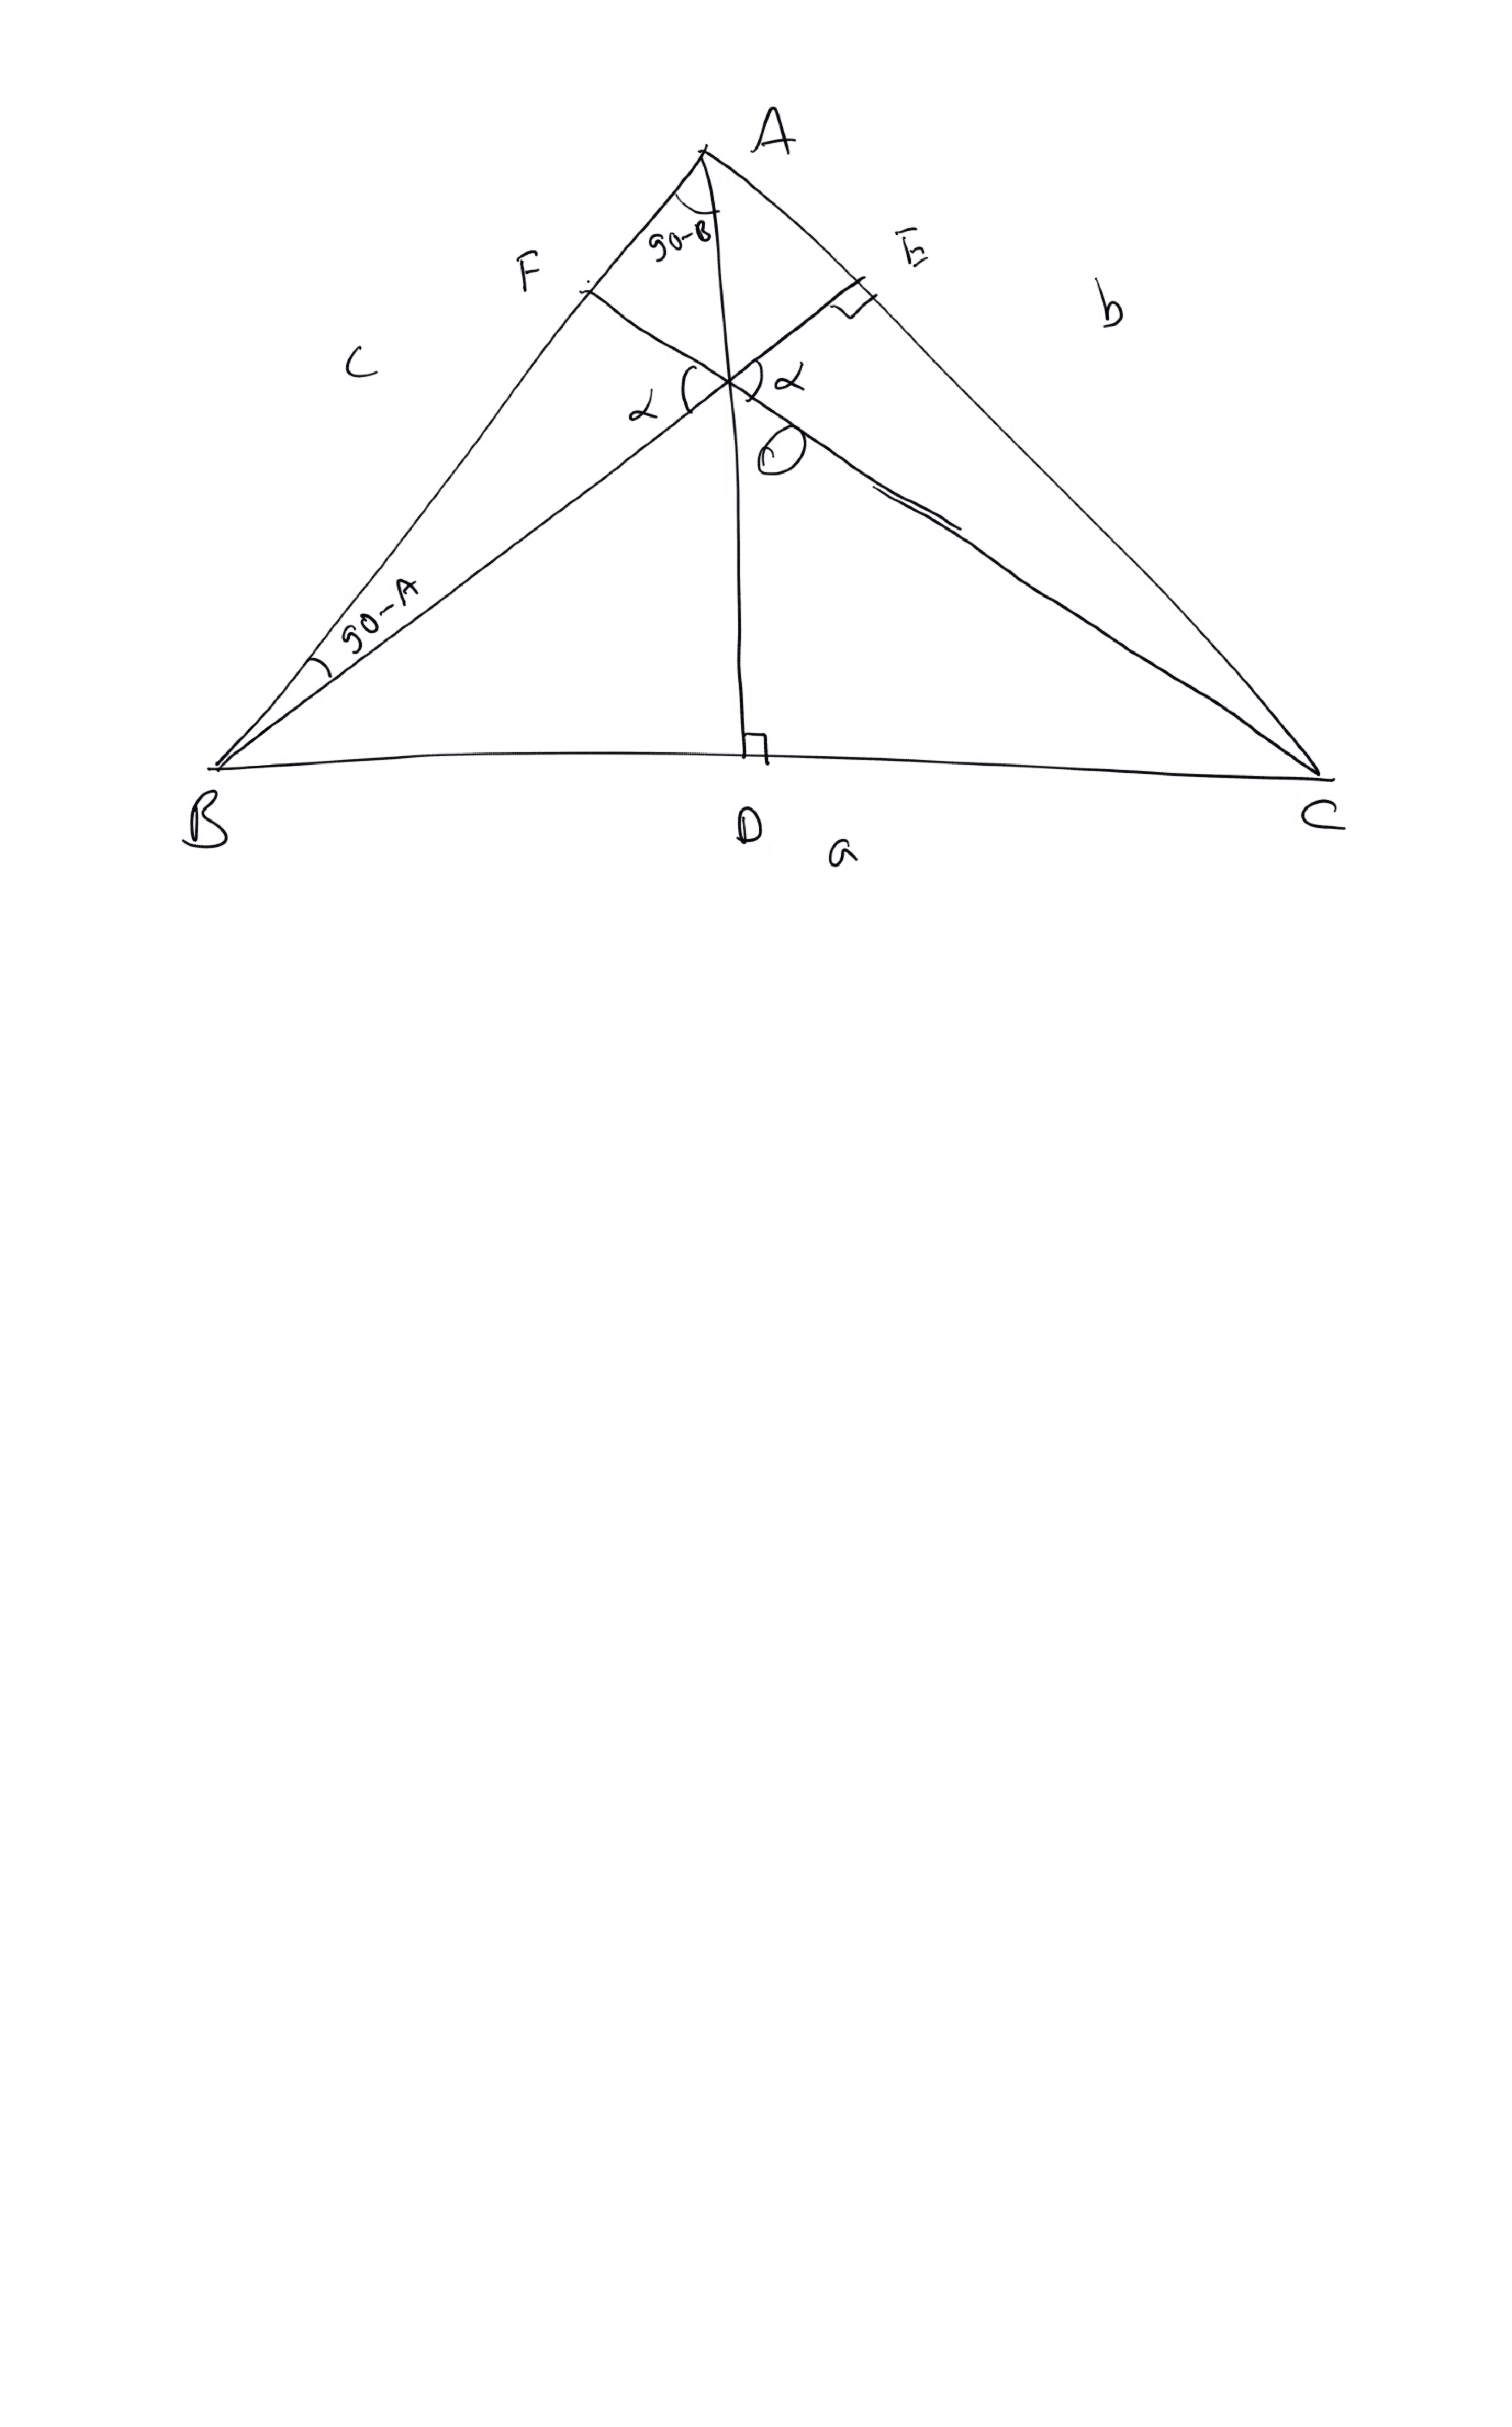
\includegraphics[width=\columnwidth]{./figs/ch3_perp_triang}
			%\vspace*{-10cm}
			\resizebox{\columnwidth}{!}{\begin{tikzpicture}
[scale=2,>=stealth,point/.style={draw,circle,fill = black,inner sep=0.5pt},]

\node (E) at (1.5, 1.5)[point,label=above :$E$] {};
\node (F) at (-1.5, 1.5)[point,label=above :$F$] {};
\node (A) at (0, 3)[point,label=above :$A$]{};
\node (B) at (-3, 0)[point,label=below left:$B$]{};
\node (C) at (3, 0)[point,label=below right:$C$]{};
\node (O) at (0,1)[point,label=above right :$O$] {};
\node (D) at (0,0)[point,label=below :$D$] {};


\draw (B)--(A);
\draw (A)--(C);
\draw (B)--(E);
\draw (C)--(F);
\draw (B)--(C);
\draw (A)--(D);

\node [below] at (0,-0.3) {$a$};
\node [above] at (-1.7,1.7) {$c$};
\node [above] at (1.7,1.7) {$b$};
\node [above] at (1,1.3) {$p$};
\node [above] at (-1,1.3) {$q$};
\node [above] at (-2.3,0.24){\rotatebox{45}{$90-A$}};
\node [above] at (-0.4,2.1) {\rotatebox{45}{$90-B$}};
\node [above] at (0.4,2.1) {\rotatebox{-45}{$90-C$}};

\tkzMarkAngle[size=.3](F,O,B);
\tkzMarkAngle[size=.3](C,O,E);
\tkzMarkAngle[size=.4](O,B,F);
\tkzMarkAngle[size=.2](F,A,O);
\tkzMarkAngle[size=.3](O,A,E);
\draw (-0.5,1) node{$\alpha$};
\draw (0.5,1) node{$\alpha$};

\end{tikzpicture}
}
		\end{center}
		\caption{Perpendiculars from vertex to opposite side meet at a point}
		\label{ch3_perp_triang}	
	\end{figure}
%
\solution In $\triangle$ s $AEB$ and $AEO$,
%
\begin{align}
AE &= c \cos A \\
OE &= AE \tan \brak{90^{\degree} - C} \brak{\because ADC \text{ is right angled}} \\
&= AE \cot C
\end{align}
%
From both the above, we get the desired result.
%
\item
	Show that $\alpha = A$.

\solution In $\triangle OEC$,
%
\begin{equation}
CE = a \cos C \brak{\because BEC \text{ is right angled}}
\end{equation}
%
Hence,
%
\begin{equation}
\begin{split}
\tan \alpha &= \frac{CE}{OE} \\
&=  \frac{a \cos C}{c \cos A \cot C} \\
&=  \frac{a \cos C \sin C}{c \cos A \cos C} \\
&= \frac{a \sin C}{c \cos A } \\
&= \frac{c \sin A}{c \cos A } \brak{\because \frac{a}{\sin A} = \frac{c}{\sin C}}\\
&= \tan A\\
\Rightarrow \alpha = A
\end{split}
\end{equation}
%
\item
	Show that $CF \perp AB$

\solution Consider triangle OFB and the result of the previous problem.  $\because$ the sum of the angles of a triangle is $180^{\degree}$, $\angle CFB = 90^{\degree}$.
{\em Conclusion: The perperdiculars from the vertex of a triangle to the opposite side meet at a point.}
\end{enumerate}
